    
\chapter{Phonology I}

\begin{center}
\begin{Large}
第366課: Phonology I: Basic Information 
\end{Large}
\end{center}
 
\par{ In this first introductory lesson to the study of Japanese phonology, we will go over the vowels in great detail. Though dialectical and historical information create a more correct and bigger picture for Japanese as a whole, we will refrain from focusing on these details at this time and focus primarily on Standard Japanese phonology. }

\par{ Some new terminology will be necessary to properly study phonology. Another thing that must be understood is that the use of \textbf{IPA }--International Phonetic Alphabet--symbols will be necessary in transcribing Japanese at this point. Symbols will be explained, but there will be no wavering in their implementation. }

\par{\textbf{Curriculum Note }: This lesson is under the process of being remodeled to only discuss vowels. So, please forgive me for its current status as a stub article. }
      
\section{Vowels}
 
\par{ The Japanese vowel space is significantly less complex than any variety of English.  If we were to map the Japanese vowel space, it would look like the chart to the left. Now,this chart uses one ad hoc character that is not the typical IPA symbol for it so that you at least know at this point that the Japanese u is still not the English u. 
\begin{figure}[h]
\centering

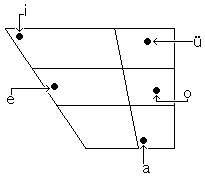
\includegraphics[width=0.9\textwidth]{figs/第08章/第366課:_japanesephonology_fig/Vowel_chart.png}

\end{figure}
}

\par{The Japanese \slash a\slash  is rather low like in English, but it is pronunciation wise a central vowel (though the phonology treats it as a back vowel). The Japanese \slash i\slash  is very similar to English. However, there is no lip spreading like there is for English speakers, and because Japanese phonology has no tense and lax distinction for high vowels like English does (beat vs bit), the actual value of a Japanese \slash i\slash  could easily sometimes sound like an "ih" to English speakers. }

\par{What do we mean by low and high and front and back? The diagram to the left is a rough representation of the vowel space inside your mouth and the position of your tongue. High vowels are made with your tongue high and the opposite is true for low vowels, and in between are mid vowels. Your tongue is raised to the back for back vowels and in the front for front vowels and in the center for central vowels. }

\par{The high-back vowel in Japanese is unrounded and if there is any lip protrusion it is actually lip compression, very similar to the Japanese \slash w\slash . [ɯᵝ] is the correct IPA notation for this sound. For speakers outside of East Japan, this vowel is actually closer to [u]. Meaning, there is lip rounding and it is then almost identical to the English vowel. However, this is not the case for Standard Japanese spoken in Tokyo and surrounding areas. }

\par{Aside from the positions being slightly different, the Japanese \slash e\slash  and \slash o\slash  are not that much different. Though, one important detail to not overlook is that these vowels are never diphthongized in Japanese. Meaning, when you pronounce them, the vowel quality is maintained and does not shift to another vowel in the vowel space. This is obligatory for many vowels in English but it is forbidden for all vowels in Japanese. This is something that English speakers in particular have a problem with understanding and should be something that you take especial attention to. }

\par{ \textbf{Time and Quality }}

\par{Japanese vowels are usually always pronounced as monophthongs because they essentially remain unchanged. The word "eye" was used as an example to find an equivalent to あ. However, the word "eye" is pronounced as a diphthong and the Japanese vowel is only equivalent to that sound's onset. Diphthongization does exist to an extent in Japanese. For example, the combination あい is often not so moraic and resembles a diphthong depending on the speaker. To test whether this is true or not, you would have to examine individual speaker variation. }
 
\par{Long vowels are treated as two separate morae. Pitch often rises or falls in long vowels. Vowel sequences are also not spoken as one unit for the same reason. Morae are ideally supposed to be spoken with the \textbf{same amount of time }. However, っ, a moraic obstruent, disrupts this and causes a pause and intensification of the following phoneme. Things like the fact it's humanly impossible to exactly say each sound unit with the same time and other things like moraic obstruents, vowel length, and diphthongization make this ideal slightly unrealistic. }
 
\par{Note: Diphthongs exist in certain varieties of Japanese which will not be discussed in this lesson. }
      
\section{Elongation \& Nasalization}
 
\par{ Vowel length differences create contrast in Japanese. A long vowel is a vowel two morae long. The vowel sequence ei often becomes [e:] in Standard Japanese, and many words spelled with ou are pronounced as [o:] instead. You can find long vowels in words of all sorts of origins. }

\begin{ltabulary}{|P|P|P|}
\hline 

酢 (Vinegar) VS 吸う (To inhale) & ビル (Building) VS ビール (Beer) & 里 (Village) VS 砂糖 (Sugar) \\ \cline{1-3}

この (This) VS 効能 (Efficacy) & 外 (Outside) VS 相当 (Befitting) & 木 (Tree) VS 紀伊 (Kii) \\ \cline{1-3}

炉 (Hearth) VS 牢 (Jail) & 血 (Blood) VS 地位 (Position) & 二 (Two) VS 二位 (2nd place) \\ \cline{1-3}

\end{ltabulary}

\begin{center}
\textbf{Nasalization }
\end{center}

\par{ Technically, vowels are natural nasalized to some extent in Japanese before nasal sounds. }
ẽɴ̩ = Yen sẽɴ̩  = Line tãɴ̩  = Phlegm jã.ma = Mountain \hfill\break
kãɴ̩ = Can \hfill\break
      
\section{Devoicing}
 
\par{ High vowels are frequently devoiced in East Japanese dialects including Standard Japanese, though it is a feature almost non-existent elsewhere in Japan. Its restrictions are not that difficult to figure out, but you will need to put some thought into this to understand. }

\par{The existence of devoicing of high vowels means that there are two allophones of \slash i\slash  and \slash ɯᵝ\slash . They are represented in IPA as [i, ɯᵝ] and [i̥ ɯ̥ᵝ] repectively. The dot you see simply stands for being unvoiced. }
ki̥ta  =  North ki-da  =  Is a tree tɕi̥.ka.i  = Close ɯmi   = Sea ni.ho.ŋ̩.go   = Japanese language tsɯ.jɯ   = Rainy season \hfill\break
ki.se.tsɯ = Season ga.sɯ̥ = Gas haɕi = Bridge haɕi̥  = Chopsticks 
\par{ The rule is this: }

\begin{center}
Low pitch V[+high] \textrightarrow  V̥  \slash  C[-voice]\_ \_ \_  \{C[-voice]\} 
\end{center}

\par{ Getting to the chase, devoicing happens between two unvoiced consonants importantly not in a stressed syllable. }
    